The UFC specification dictates a certain ordering of the vertices,
edges etc. of the cells of a finite element mesh. First, an \emph{ad
hoc} ordering is picked for the vertices of each cell. Then, the
remaining entities are ordered based on a simple rule, as described in
detail below.

\section{Basic concepts}

The topological entities of a cell (or mesh) are referred to as
\emph{mesh entities}. A mesh entity can be identified by a pair
$(d, i)$, where $d$ is the topological dimension of the mesh entity and $i$
is a unique index of the mesh entity. Mesh entities are numbered
within each topological dimension from $0$ to $n_d-1$, where $n_d$ is
the number of mesh entities of topological dimension $d$.

For convenience, mesh entities of topological dimension $0$ are
referred to as \emph{vertices}, entities of dimension $1$
as \emph{edges}, entities of dimension $2$ as \emph{faces}, entities of
\emph{codimension} $1$ as \emph{facets} and entities of codimension
$0$ as \emph{cells}. These concepts are summarized in
Table~\ref{tab:entities}.

Thus, the vertices of a tetrahedron are identified as
$v_0 = (0, 0)$, $v_1 = (0, 1)$ and $v_2 = (0, 2)$,
the edges are
$e_0 = (1, 0)$, $e_1 = (1, 1)$, $e_2 = (1, 2)$,
$e_3 = (1, 3)$, $e_4 = (1, 4)$ and $e_5 = (1, 5)$,
the faces (facets) are
$f_0 = (2, 0)$, $f_1 = (2, 1)$, $f_2 = (2, 2)$ and $f_3 = (2, 3)$,
and the cell itself is
$c_0 = (3, 0)$.

\begin{table}[H]
\linespread{1.2}\selectfont
  \begin{center}
    \begin{tabular}{|l|c|c|}
      \hline
      Entity & Dimension & Codimension \\
      \hline
      Vertex & $0$       & -- \\
      Edge   & $1$       & -- \\
      Face   & $2$       & -- \\
      & & \\
      Facet  & --      &  $1$ \\
      Cell   & --      &  $0$ \\
      \hline
    \end{tabular}
    \caption{Named mesh entities.}
    \label{tab:entities}
  \end{center}
\end{table}

\section{Numbering of vertices}

For simplicial cells (intervals, triangles and tetrahedra) of a finite
element mesh, the vertices are numbered locally based on the
corresponding global vertex numbers. In particular, a tuple of
increasing local vertex numbers corresponds to a tuple of increasing
global vertex numbers.  This is illustrated in
Figure~\ref{fig:numbering_example_triangles} for a mesh consisting of
two triangles.
 
\begin{figure}[htbp]
  \begin{center}
    \psfrag{v0}{$v_0$}
    \psfrag{v1}{$v_1$}
    \psfrag{v2}{$v_2$}
    \psfrag{0}{$0$}
    \psfrag{1}{$1$}
    \psfrag{2}{$2$}
    \psfrag{3}{$3$}
    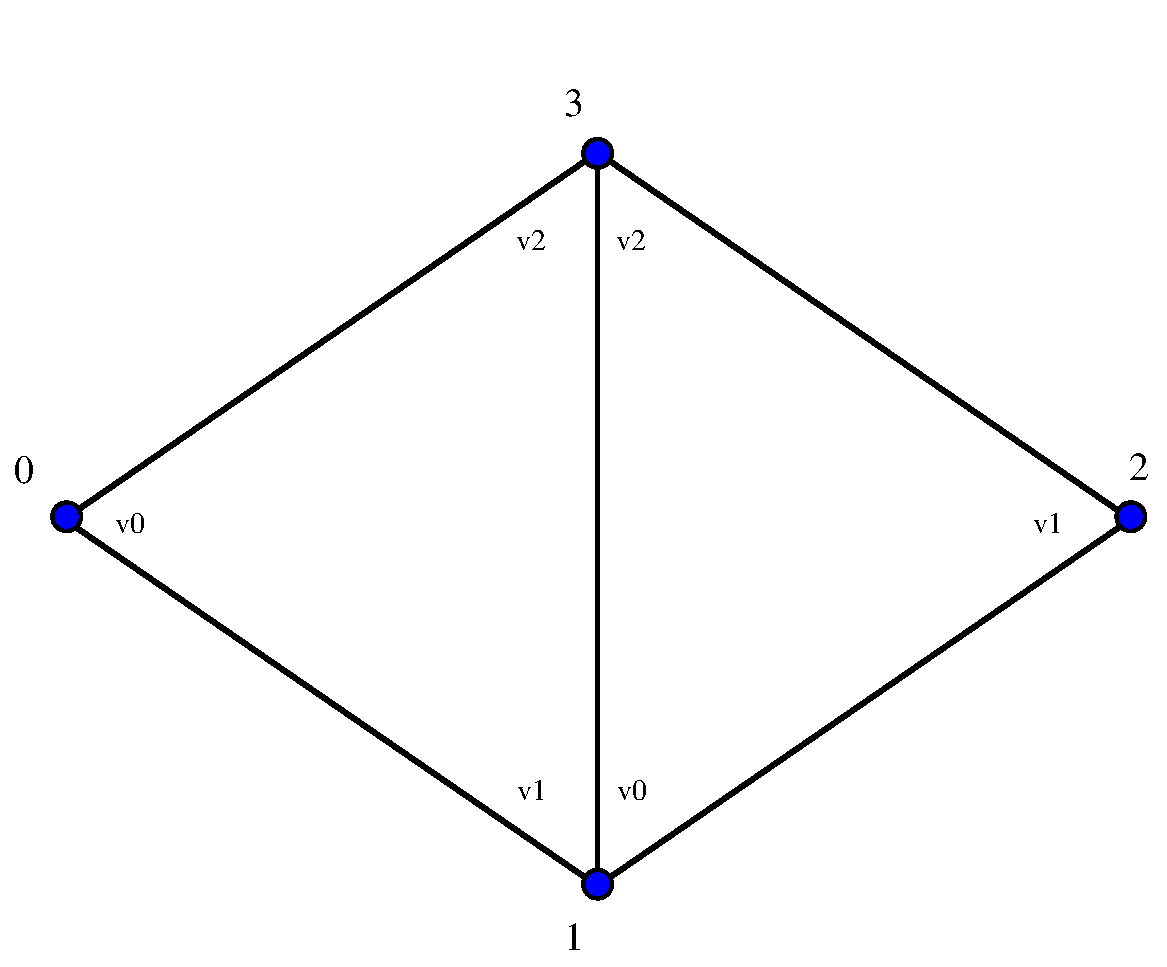
\includegraphics[width=8cm]{eps/numbering_example_triangles.eps}
    \caption{The vertices of a simplicial mesh are numbered locally
      based on the corresponding global vertex numbers.}
    \label{fig:numbering_example_triangles}
  \end{center}
\end{figure}

For non-simplicial cells (quadrilaterals and hexahedra), the ordering
is arbitrary, as long as each cell is isomorphic to the corresponding
reference cell by matching each vertex with the corresponding vertex
in the reference cell. This is illustrated in
Figure~\ref{fig:numbering_example_quadrilaterals} for a mesh
consisting of two quadrilaterals.

\begin{figure}[htbp]
  \begin{center}
    \psfrag{v0}{$v_0$}
    \psfrag{v1}{$v_1$}
    \psfrag{v2}{$v_2$}
    \psfrag{v3}{$v_3$}
    \psfrag{0}{$0$}
    \psfrag{1}{$1$}
    \psfrag{2}{$2$}
    \psfrag{3}{$3$}
    \psfrag{4}{$4$}
    \psfrag{5}{$5$}
    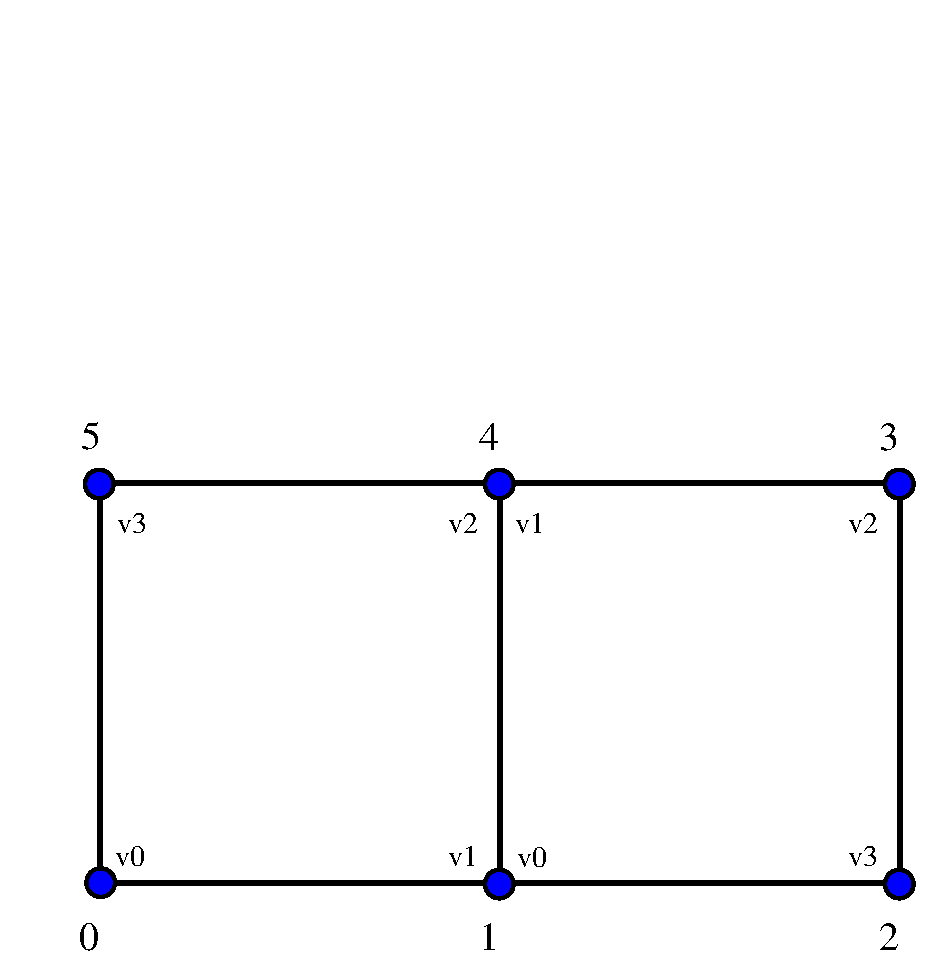
\includegraphics[width=8cm]{eps/numbering_example_quadrilaterals.eps}
    \caption{The local numbering of vertices of a non-simplicial mesh
      is arbitrary, as long as each cell is isomorphic to the
      reference cell by matching each vertex to the corresponding
      vertex of the reference cell.}
    \label{fig:numbering_example_quadrilaterals}
  \end{center}
\end{figure}

\section{Numbering of remaining mesh entities}

When the vertices have been numbered, the remaining mesh entities are
numbered within each topological dimension based on a
\emph{lexicographical ordering} of the corresponding ordered tuples of
\emph{non-incident vertices}.

As an illustration, consider the numbering of edges (the mesh entities
of topological dimension one) on the reference triangle in
Figure~\ref{fig:orderingexample,triangle}. To number the edges of the
reference triangle, we identify for each edge the corresponding
non-incident vertices. For each edge, there is only one such vertex
(the vertex opposite to the edge). We thus identify the three edges in
the reference triangle with the tuples $(v_0)$, $(v_1)$ and $(v_2)$. The
first of these is edge $e_0$ between vertices $v_1$ and $v_2$ opposite
to vertex $v_0$, the second is edge $e_1$ between vertices $v_0$ and
$v_2$ opposite to vertex $v_1$, and the third is edge $e_2$ between
vertices $v_0$ and $v_1$ opposite to vertex $v_2$.

Similarly, we identify the six edges of the reference tetrahedron with
the corresponding non-incident tuples $(v_0, v_1)$, $(v_0, v_2)$,
$(v_0, v_3)$, $(v_1, v_2)$, $(v_1, v_3)$ and $(v_2, v_3)$. The first of these is
edge $e_0$ between vertices $v_2$ and $v_3$ opposite to vertices $v_0$
and $v_1$ as shown in Figure~\ref{fig:orderingexample,tetrahedron}.

\begin{figure}[htbp]
  \begin{center}
    \psfrag{v0}{$v_0$}
    \psfrag{v1}{$v_1$}
    \psfrag{v2}{$v_2$}
    \psfrag{e0}{$e_0$}
    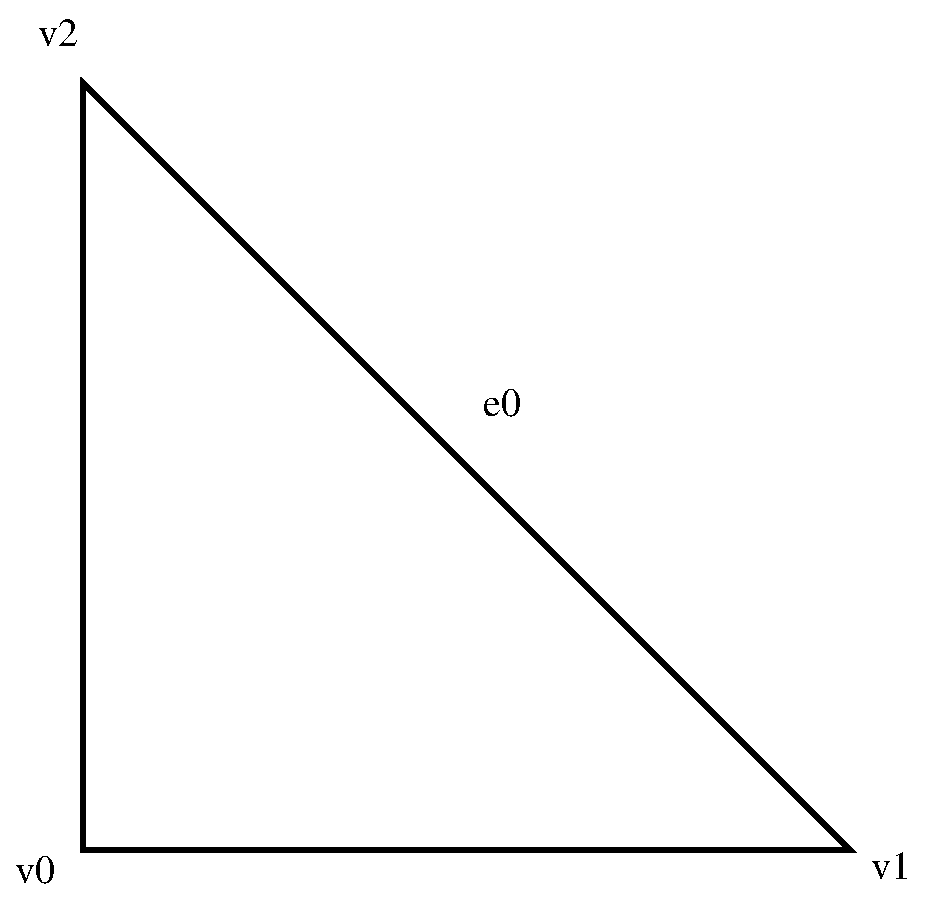
\includegraphics[width=5cm]{eps/ordering_example_triangle.eps}
    \caption{Mesh entities are ordered based on a lexicographical ordering
      of the corresponding ordered tuples of non-incident vertices.
      The first edge $e_0$ is non-incident to vertex $v_0$.}
    \label{fig:orderingexample,triangle}
  \end{center}
\end{figure}

\begin{figure}[htbp]
  \begin{center}
    \psfrag{v0}{$v_0$}
    \psfrag{v1}{$v_1$}
    \psfrag{v2}{$v_2$}
    \psfrag{v3}{$v_3$}
    \psfrag{e0}{$e_0$}
    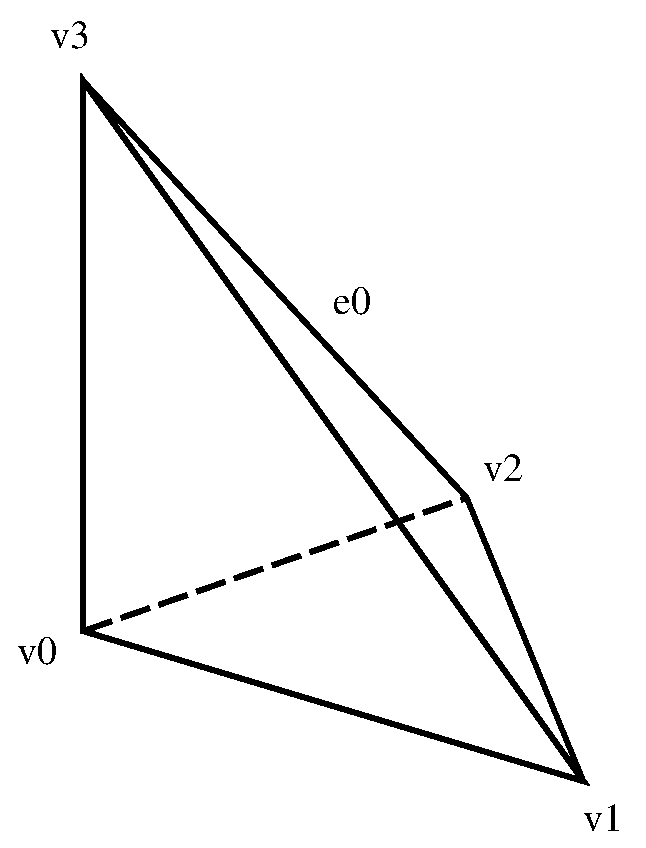
\includegraphics[width=5cm]{eps/ordering_example_tetrahedron.eps}
    \caption{Mesh entities are ordered based on a lexicographical ordering
      of the corresponding ordered tuples of non-incident vertices.
      The first edge $e_0$ is non-incident to vertices $v_0$ and $v_1$.}
    \label{fig:orderingexample,tetrahedron}
  \end{center}
\end{figure}

\subsection{Relative ordering}

The relative ordering of mesh entities with respect to other incident
mesh entities follows by sorting the entities by their (local)
indices. Thus, the pair of vertices incident to the first edge $e_0$
of a triangular cell is $(v_1, v_2)$, not $(v_2, v_1)$. Similarly, the
first face $f_0$ of a tetrahedral cell is incident to vertices $(v_1,
v_2, v_3)$.

For simplicial cells, the relative ordering in combination with the
convention of numbering the vertices locally based on global vertex
indices means that two incident cells will always agree on the
orientation of incident sub simplices. Thus, two incident triangles
will agree on the orientation of the common edge and two incident
tetrahedra will agree on the orientation of the common edge(s) and the
orientation of the common face (if any). This is illustrated in
Figure~\ref{fig:orientation_example_triangles} for two incident
triangles sharing a common edge.

\begin{figure}[htbp]
  \begin{center}
    \psfrag{v0}{$v_0$}
    \psfrag{v1}{$v_1$}
    \psfrag{v2}{$v_2$}
    \psfrag{v3}{$v_3$}
    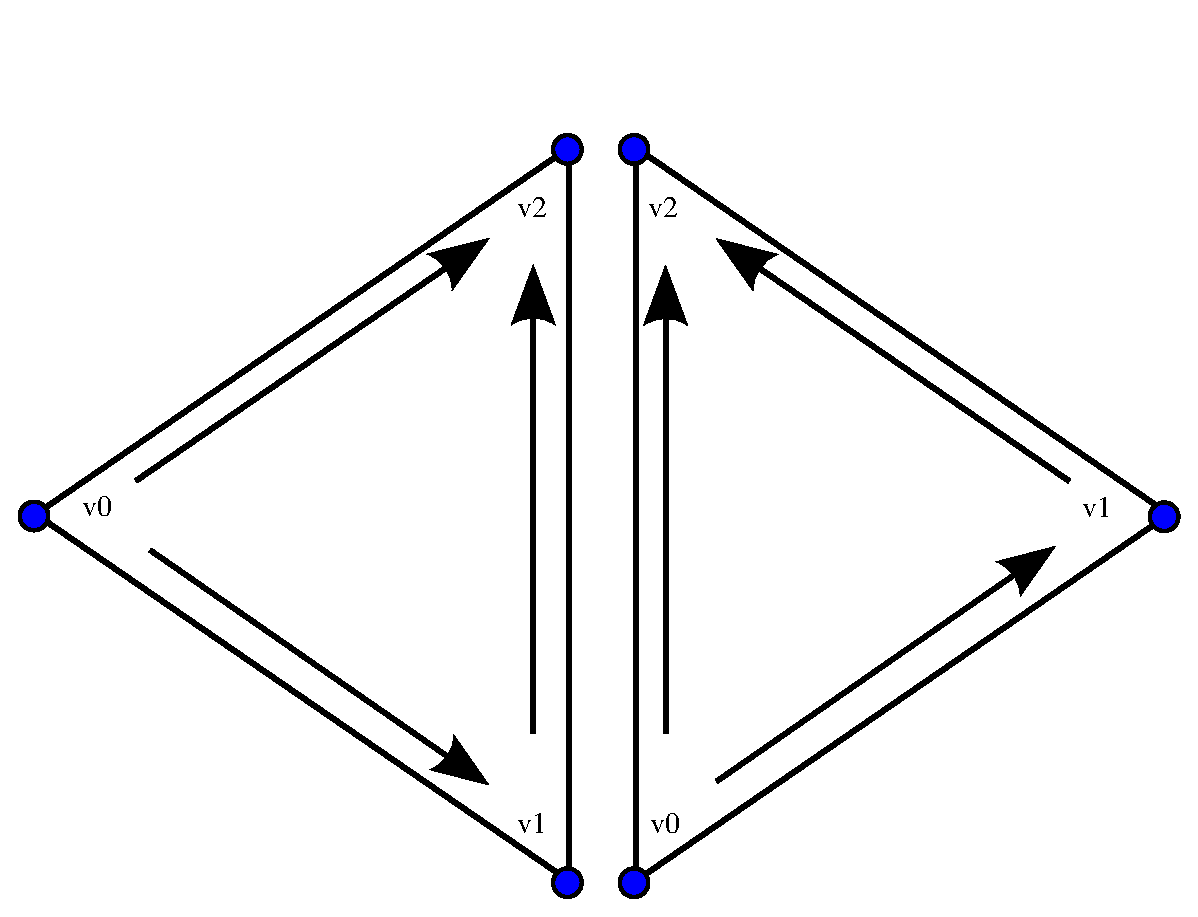
\includegraphics[width=9cm]{eps/orientation_example_triangles.eps}
    \caption{Two incident triangles will always agree on the
      orientation of the common edge.}
    \label{fig:orientation_example_triangles}
  \end{center}
\end{figure}

\subsection{Limitations}
 
The UFC specification is only concerned with the ordering of mesh
entities with respect to entities of larger topological dimension. In
other words, the UFC specification is only concerned with the ordering
of incidence relations of the class $d - d'$ where $d > d'$. For
example, the UFC specification is not concerned with the ordering of
incidence relations of the class $0 - 1$, that is, the ordering of
edges incident to vertices.

\newpage

\section{Numbering for reference cells}

The numbering scheme is demonstrated below for cells
isomorphic to each of the five reference cells.

\subsection{Numbering for intervals}

\begin{table}[H]
\linespread{1.2}\selectfont
  \begin{center}
    \begin{tabular}{|c|c|c|}
      \hline
      Entity & Incident vertices & Non-incident vertices \\
      \hline
      \hline
      $v_0 = (0, 0)$ & $(v_0)$ & $(v_1)$ \\
      \hline
      $v_1 = (0, 1)$ & $(v_1)$ & $(v_0)$ \\
      \hline
      $c_0 = (1, 0)$ & $(v_0, v_1)$ & $\emptyset$ \\
      \hline
    \end{tabular}
    \caption{Numbering of mesh entities on intervals.}
    \label{tab:interval,entities}
  \end{center}
\end{table}

\subsection{Numbering for triangular cells}

\begin{table}[H]
\linespread{1.2}\selectfont
  \begin{center}
    \begin{tabular}{|c|c|c|}
      \hline
      Entity & Incident vertices & Non-incident vertices \\
      \hline
      \hline
      $v_0 = (0, 0)$ & $(v_0)$ & $(v_1, v_2)$ \\
      \hline
      $v_1 = (0, 1)$ & $(v_1)$ & $(v_0, v_2)$ \\
      \hline
      $v_2 = (0, 2)$ & $(v_2)$ & $(v_0, v_1)$ \\
      \hline
      $e_0 = (1, 0)$ & $(v_1, v_2)$ & $(v_0)$ \\
      \hline
      $e_1 = (1, 1)$ & $(v_0, v_2)$ & $(v_1)$ \\
      \hline
      $e_2 = (1, 2)$ & $(v_0, v_1)$ & $(v_2)$ \\
      \hline
      $c_0 = (2, 0)$ & $(v_0, v_1, v_2)$ & $\emptyset$ \\
      \hline
    \end{tabular}
    \caption{Numbering of mesh entities on triangular cells.}
    \label{tab:triangle,entities}
  \end{center}
\end{table}

\subsection{Numbering for quadrilateral cells}

\begin{table}[H]
\linespread{1.1}\selectfont
  \begin{center}
    \begin{tabular}{|c|c|c|}
      \hline
      Entity & Incident vertices & Non-incident vertices \\
      \hline
      \hline
      $v_0 = (0, 0)$ & $(v_0)$ & $(v_1, v_2, v_3)$ \\
      \hline
      $v_1 = (0, 1)$ & $(v_1)$ & $(v_0, v_2, v_3)$ \\
      \hline
      $v_2 = (0, 2)$ & $(v_2)$ & $(v_0, v_1, v_3)$ \\
      \hline
      $v_3 = (0, 3)$ & $(v_3)$ & $(v_0, v_1, v_2)$ \\
      \hline
      $e_0 = (1, 0)$ & $(v_2, v_3)$ & $(v_0, v_1)$ \\
      \hline
      $e_1 = (1, 1)$ & $(v_1, v_2)$ & $(v_0, v_3)$ \\
      \hline
      $e_2 = (1, 2)$ & $(v_0, v_3)$ & $(v_1, v_2)$ \\
      \hline
      $e_3 = (1, 3)$ & $(v_0, v_1)$ & $(v_2, v_3)$ \\
      \hline
      $c_0 = (2, 0)$ & $(v_0, v_1, v_2, v_3)$ & $\emptyset$ \\
      \hline
    \end{tabular}
    \caption{Numbering of mesh entities on quadrilateral cells.}
    \label{tab:quadrilateral,entities}
  \end{center}
\end{table}

\newpage

\subsection{Numbering for tetrahedral cells}

\begin{table}[H]
\linespread{1.1}\selectfont
  \begin{center}
    \begin{tabular}{|c|c|c|}
      \hline
      Entity & Incident vertices & Non-incident vertices \\
      \hline
      \hline
      $v_0 = (0, 0)$ & $(v_0)$ & $(v_1, v_2, v_3)$ \\
      \hline
      $v_1 = (0, 1)$ & $(v_1)$ & $(v_0, v_2, v_3)$ \\
      \hline
      $v_2 = (0, 2)$ & $(v_2)$ & $(v_0, v_1, v_3)$ \\
      \hline
      $v_3 = (0, 3)$ & $(v_3)$ & $(v_0, v_1, v_2)$ \\
      \hline
      $e_0 = (1, 0)$ & $(v_2, v_3)$ & $(v_0, v_1)$ \\
      \hline
      $e_1 = (1, 1)$ & $(v_1, v_3)$ & $(v_0, v_2)$ \\
      \hline
      $e_2 = (1, 2)$ & $(v_1, v_2)$ & $(v_0, v_3)$ \\
      \hline
      $e_3 = (1, 3)$ & $(v_0, v_3)$ & $(v_1, v_2)$ \\
      \hline
      $e_4 = (1, 4)$ & $(v_0, v_2)$ & $(v_1, v_3)$ \\
      \hline
      $e_5 = (1, 5)$ & $(v_0, v_1)$ & $(v_2, v_3)$ \\
      \hline
      $f_0 = (2, 0)$ & $(v_1, v_2, v_3)$ & $(v_0)$ \\
      \hline
      $f_1 = (2, 1)$ & $(v_0, v_2, v_3)$ & $(v_1)$ \\
      \hline
      $f_2 = (2, 2)$ & $(v_0, v_1, v_3)$ & $(v_2)$ \\
      \hline
      $f_3 = (2, 3)$ & $(v_0, v_1, v_2)$ & $(v_3)$ \\
      \hline
      $c_0 = (3, 0)$ & $(v_0, v_1, v_2, v_3)$ & $\emptyset$ \\
      \hline
    \end{tabular}
    \caption{Numbering of mesh entities on tetrahedral cells.}
        \label{tab:tetrahedron,entities} 
  \end{center}
\end{table}

\vfill

\newpage

\subsection{Numbering for hexahedral cells}

\vspace{-0.5cm}
\begin{table}[H]
\small
\linespread{1.2}\selectfont
  \begin{center}
    \begin{tabular}{|c|c|c|}
      \hline
      Entity & Incident vertices & Non-incident vertices \\
      \hline
      \hline
      $v_0 = (0, 0)$ & $(v_0)$ & $(v_1, v_2, v_3, v_4, v_5, v_6, v_7)$ \\
      \hline
      $v_1 = (0, 1)$ & $(v_1)$ & $(v_0, v_2, v_3, v_4, v_5, v_6, v_7)$ \\
      \hline
      $v_2 = (0, 2)$ & $(v_2)$ & $(v_0, v_1, v_3, v_4, v_5, v_6, v_7)$ \\
      \hline
      $v_3 = (0, 3)$ & $(v_3)$ & $(v_0, v_1, v_2, v_4, v_5, v_6, v_7)$ \\
      \hline
      $v_4 = (0, 4)$ & $(v_4)$ & $(v_0, v_1, v_2, v_3, v_5, v_6, v_7)$ \\
      \hline
      $v_5 = (0, 5)$ & $(v_5)$ & $(v_0, v_1, v_2, v_3, v_4, v_6, v_7)$ \\
      \hline
      $v_6 = (0, 6)$ & $(v_6)$ & $(v_0, v_1, v_2, v_3, v_4, v_5, v_7)$ \\
      \hline
      $v_7 = (0, 7)$ & $(v_7)$ & $(v_0, v_1, v_2, v_3, v_4, v_5, v_6)$ \\
      \hline
      $e_0 = (1, 0)$ & $(v_6, v_7)$ & $(v_0, v_1, v_2, v_3, v_4, v_5)$ \\
      \hline
      $e_1 = (1, 1)$ & $(v_5, v_6)$ & $(v_0, v_1, v_2, v_3, v_4, v_7)$ \\
      \hline
      $e_2 = (1, 2)$ & $(v_4, v_7)$ & $(v_0, v_1, v_2, v_3, v_5, v_6)$ \\
      \hline
      $e_3 = (1, 3)$ & $(v_4, v_5)$ & $(v_0, v_1, v_2, v_3, v_6, v_7)$ \\
      \hline
      $e_4 = (1, 4)$ & $(v_3, v_7)$ & $(v_0, v_1, v_2, v_4, v_5, v_6)$ \\
      \hline
      $e_5 = (1, 5)$ & $(v_2, v_6)$ & $(v_0, v_1, v_3, v_4, v_5, v_7)$ \\
      \hline
      $e_6 = (1, 6)$ & $(v_2, v_3)$ & $(v_0, v_1, v_4, v_5, v_6, v_7)$ \\
      \hline
      $e_7 = (1, 7)$ & $(v_1, v_5)$ & $(v_0, v_2, v_3, v_4, v_6, v_7)$ \\
      \hline
      $e_8 = (1, 8)$ & $(v_1, v_2)$ & $(v_0, v_3, v_4, v_5, v_6, v_7)$ \\
      \hline
      $e_9 = (1, 9)$ & $(v_0, v_4)$ & $(v_1, v_2, v_3, v_5, v_6, v_7)$ \\
      \hline
      $e_{10} = (1, 10)$ & $(v_0, v_3)$ & $(v_1, v_2, v_4, v_5, v_6, v_7)$ \\
      \hline
      $e_{11} = (1, 11)$ & $(v_0, v_1)$ & $(v_2, v_3, v_4, v_5, v_6, v_7)$ \\
      \hline
      $f_0 = (2, 0)$ & $(v_4, v_5, v_6, v_7)$ & $(v_0, v_1, v_2, v_3)$ \\
      \hline
      $f_1 = (2, 1)$ & $(v_2, v_3, v_6, v_7)$ & $(v_0, v_1, v_4, v_5)$ \\
      \hline
      $f_2 = (2, 2)$ & $(v_1, v_2, v_5, v_6)$ & $(v_0, v_3, v_4, v_7)$ \\
      \hline
      $f_3 = (2, 3)$ & $(v_0, v_3, v_4, v_7)$ & $(v_1, v_2, v_5, v_6)$ \\
      \hline
      $f_4 = (2, 4)$ & $(v_0, v_1, v_4, v_5)$ & $(v_2, v_3, v_6, v_7)$ \\
      \hline
      $f_5 = (2, 5)$ & $(v_0, v_1, v_2, v_3)$ & $(v_4, v_5, v_6, v_7)$ \\
      \hline
      $c_0 = (3, 0)$ & $(v_0, v_1, v_2, v_3, v_4, v_5, v_6, v_7)$ & $\emptyset$ \\
      \hline
    \end{tabular}
    \caption{Numbering of mesh entities on hexahedral cells.}
    \label{tab:hexahedron,entities}
  \end{center}
\end{table}
